% (find-LATEX "2022-2-C3-topologia.tex")
% (defun c () (interactive) (find-LATEXsh "lualatex -record 2022-2-C3-topologia.tex" :end))
% (defun C () (interactive) (find-LATEXsh "lualatex 2022-2-C3-topologia.tex" "Success!!!"))
% (defun D () (interactive) (find-pdf-page      "~/LATEX/2022-2-C3-topologia.pdf"))
% (defun d () (interactive) (find-pdftools-page "~/LATEX/2022-2-C3-topologia.pdf"))
% (defun e () (interactive) (find-LATEX "2022-2-C3-topologia.tex"))
% (defun o () (interactive) (find-LATEX "2021-1-C3-abertos-e-fechados.tex"))
% (defun u () (interactive) (find-latex-upload-links "2022-2-C3-topologia"))
% (defun v () (interactive) (find-2a '(e) '(d)))
% (defun d0 () (interactive) (find-ebuffer "2022-2-C3-topologia.pdf"))
% (defun cv () (interactive) (C) (ee-kill-this-buffer) (v) (g))
%          (code-eec-LATEX "2022-2-C3-topologia")
% (find-pdf-page   "~/LATEX/2022-2-C3-topologia.pdf")
% (find-sh0 "cp -v  ~/LATEX/2022-2-C3-topologia.pdf /tmp/")
% (find-sh0 "cp -v  ~/LATEX/2022-2-C3-topologia.pdf /tmp/pen/")
%     (find-xournalpp "/tmp/2022-2-C3-topologia.pdf")
%   file:///home/edrx/LATEX/2022-2-C3-topologia.pdf
%               file:///tmp/2022-2-C3-topologia.pdf
%           file:///tmp/pen/2022-2-C3-topologia.pdf
% http://angg.twu.net/LATEX/2022-2-C3-topologia.pdf
% (find-LATEX "2019.mk")
% (find-sh0 "cd ~/LUA/; cp -v Pict2e1.lua Pict2e1-1.lua Piecewise1.lua ~/LATEX/")
% (find-sh0 "cd ~/LUA/; cp -v Pict2e1.lua Pict2e1-1.lua Pict3D1.lua ~/LATEX/")
% (find-sh0 "cd ~/LUA/; cp -v C2Subst1.lua C2Formulas1.lua ~/LATEX/")
% (find-CN-aula-links "2022-2-C3-topologia" "3" "c3m222top" "c3to")

% «.defs»			(to "defs")
% «.title»			(to "title")
% «.links»			(to "links")
% «.interior»			(to "interior")
% «.infinitas-bob»		(to "infinitas-bob")
% «.exercicio-5»		(to "exercicio-5")
% «.exercicio-6»		(to "exercicio-6")
% «.fecho»			(to "fecho")
% «.exercicio-7»		(to "exercicio-7")
% «.algumas-traducoes»		(to "algumas-traducoes")
% «.algumas-nots-novas»		(to "algumas-nots-novas")
% «.maximos-numa-elipse»	(to "maximos-numa-elipse")
%
% «.djvuize»		(to "djvuize")



% <videos>
% Video (not yet):
% (find-ssr-links     "c3m222top" "2022-2-C3-topologia")
% (code-eevvideo      "c3m222top" "2022-2-C3-topologia")
% (code-eevlinksvideo "c3m222top" "2022-2-C3-topologia")
% (find-c3m222topvideo "0:00")

\documentclass[oneside,12pt]{article}
\usepackage[colorlinks,citecolor=DarkRed,urlcolor=DarkRed]{hyperref} % (find-es "tex" "hyperref")
\usepackage{amsmath}
\usepackage{amsfonts}
\usepackage{amssymb}
\usepackage{pict2e}
\usepackage[x11names,svgnames]{xcolor} % (find-es "tex" "xcolor")
\usepackage{colorweb}                  % (find-es "tex" "colorweb")
%\usepackage{tikz}
%
% (find-dn6 "preamble6.lua" "preamble0")
%\usepackage{proof}   % For derivation trees ("%:" lines)
%\input diagxy        % For 2D diagrams ("%D" lines)
%\xyoption{curve}     % For the ".curve=" feature in 2D diagrams
%
\usepackage{edrx21}               % (find-LATEX "edrx21.sty")
\input edrxaccents.tex            % (find-LATEX "edrxaccents.tex")
\input edrx21chars.tex            % (find-LATEX "edrx21chars.tex")
\input edrxheadfoot.tex           % (find-LATEX "edrxheadfoot.tex")
\input edrxgac2.tex               % (find-LATEX "edrxgac2.tex")
%\usepackage{emaxima}              % (find-LATEX "emaxima.sty")
%
% (find-es "tex" "geometry")
\usepackage[a6paper, landscape,
            top=1.5cm, bottom=.25cm, left=1cm, right=1cm, includefoot
           ]{geometry}
%
\begin{document}

\catcode`\^^J=10
\directlua{dofile "dednat6load.lua"}  % (find-LATEX "dednat6load.lua")
%L dofile "Piecewise1.lua"           -- (find-LATEX "Piecewise1.lua")
%L dofile "QVis1.lua"                -- (find-LATEX "QVis1.lua")
%L dofile "Pict3D1.lua"              -- (find-LATEX "Pict3D1.lua")
%L dofile "C2Formulas1.lua"          -- (find-LATEX "C2Formulas1.lua")
%L Pict2e.__index.suffix = "%"
\pu
\def\pictgridstyle{\color{GrayPale}\linethickness{0.3pt}}
\def\pictaxesstyle{\linethickness{0.5pt}}
\def\pictnaxesstyle{\color{GrayPale}\linethickness{0.5pt}}
\celllower=2.5pt

% «defs»  (to ".defs")
% (find-LATEX "edrx21defs.tex" "colors")
% (find-LATEX "edrx21.sty")

\def\u#1{\par{\footnotesize \url{#1}}}

\def\drafturl{http://angg.twu.net/LATEX/2022-2-C3.pdf}
\def\drafturl{http://angg.twu.net/2022.2-C3.html}
\def\draftfooter{\tiny \href{\drafturl}{\jobname{}} \ColorBrown{\shorttoday{} \hours}}

\def\BA{\mathsf{B}}
\def\BF{\overline{\mathsf{B}}}




%  _____ _ _   _                               
% |_   _(_) |_| | ___   _ __   __ _  __ _  ___ 
%   | | | | __| |/ _ \ | '_ \ / _` |/ _` |/ _ \
%   | | | | |_| |  __/ | |_) | (_| | (_| |  __/
%   |_| |_|\__|_|\___| | .__/ \__,_|\__, |\___|
%                      |_|          |___/      
%
% «title»  (to ".title")
% (c3m222topp 1 "title")
% (c3m222topa   "title")

\thispagestyle{empty}

\begin{center}

\vspace*{1.2cm}

{\bf \Large Cálculo 3 - 2022.2}

\bsk

Aulas 25 e 26: abertos e fechados em $\R^2$

\bsk

Eduardo Ochs - RCN/PURO/UFF

\url{http://angg.twu.net/2022.2-C3.html}

\end{center}

\newpage

% «links»  (to ".links")
% (c3m222topp 2 "links")
% (c3m222topa   "links")
% (find-tudosgrep "grep --color=auto -niH --null -e aberto *.txt")
% (c3m211afp 1 "title")
% (c3m211afa   "title")

{\bf Links}

Capítulo 4 do Bortolossi:

{\footnotesize

% (find-books "__analysis/__analysis.el" "bortolossi")
% (find-books "__analysis/__analysis.el" "bortolossi" "seis conjuntos abaixo")
% (find-bortolossi4page (+ -120 130)   "seis conjuntos abaixo")
\url{http://angg.twu.net/2019.2-C3/Bortolossi/bortolossi-cap-4.pdf}

}

\ssk

Como debugar representações gráficas:

{\footnotesize

% (c2m221isp 10 "exercicio-2-dica")
% (c2m221isa    "exercicio-2-dica")
%    http://angg.twu.net/LATEX/2022-1-C2-infs-e-sups.pdf#page=10
\url{http://angg.twu.net/LATEX/2022-1-C2-infs-e-sups.pdf#page=10}

}

\ssk

Abertos, fechados e compactos na Wikipedia:

{\footnotesize

\url{https://en.wikipedia.org/wiki/Metric_space}

\url{https://en.wikipedia.org/wiki/General_topology}

\url{https://en.wikipedia.org/wiki/Topology}

}


\ssk

Este PDF é baseado neste outro mais antigo:

{\footnotesize

% (c3m211afp 1 "title")
% (c3m211afa   "title")
%    http://angg.twu.net/LATEX/2021-1-C3-abertos-e-fechados.pdf
\url{http://angg.twu.net/LATEX/2021-1-C3-abertos-e-fechados.pdf}

}

\ssk





\newpage

{\bf Introdução}

Dê uma olhada no capítulo 4 do Bortolossi...

Comece pela seção 4.1, ``Por que funções contínuas são importantes'',

depois leia a seção 4.3, sobre o Teorema de Weirstrass em $n$ variáveis,

e relembre a definição de distância euclidiana na p.139.

\msk

Nós vamos começar entendendo as definições das páginas 142

até 148, e vamos reescrevê-las de um jeito bem mais curto.

\msk

Nós vamos ver como fazer hipóteses sobre os exercícios

dos próximos dois slides, como testar essas hipóteses,

e como descartar as hipóteses erradas.

\newpage

% «nove-subconjuntos»  (to ".nove-subconjuntos")
% (c3m211afp 3 "nove-subconjuntos")
% (c3m211afa   "nove-subconjuntos")

{\bf Nove subconjuntos de $\R^2$}

(Compare com a p.130 do Bortolossi...)


\msk

\def\eee{\text{\; e \;}}

Sejam:
%
$$\begin{array}{rcl}
  C_1 &=& \setofxyst{ 2<y≤3 }, \\
  C_2 &=& \setofxyst{ 2<y≤3 \eee 1≤x<4 }, \\
  C_3 &=& \setofxyst{   d((x,y),(1,2))≤2 }, \\
  C_4 &=& \setofxyst{ 1<d((x,y),(1,2))≤2 }, \\
  C_5 &=& \setofxyst{   d((x,y),(1,2))≤2 \eee 1<x }, \\
  C_6 &=& \setofxyst{ y>x }, \\
  \end{array}
$$


\def\vc#1{\myvcenter{#1}}

$$
  % (find-latexscan-links "C3" "20210908_C_6")
  % (find-xpdf-page "~/LATEX/2021-1-C3/20210908_C_6.pdf")
  C_7 \;=\;
  \vc{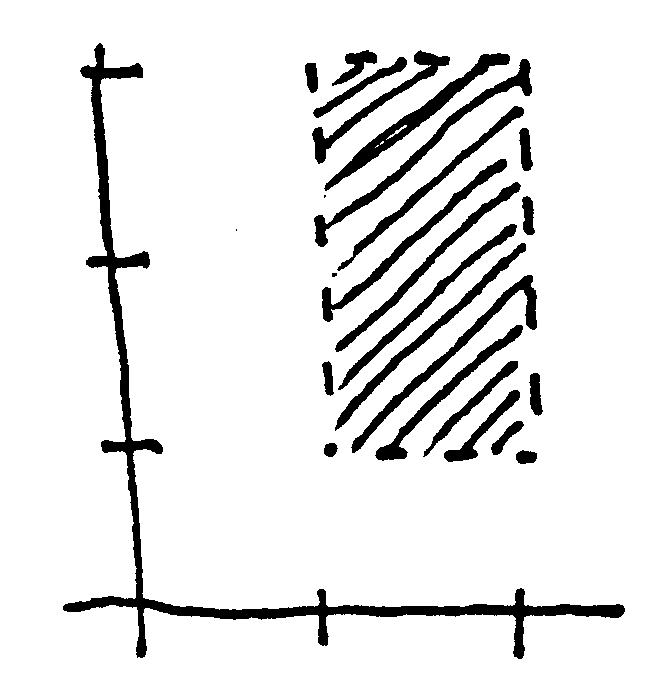
\includegraphics[height=2cm]{2021-1-C3/20210908_C_6.pdf}},
  %
  \quad
  %
  % (find-latexscan-links "C3" "20210908_C_7")
  % (find-xpdf-page "~/LATEX/2021-1-C3/20210908_C_7.pdf")
  C_8 \;=\;
  \vc{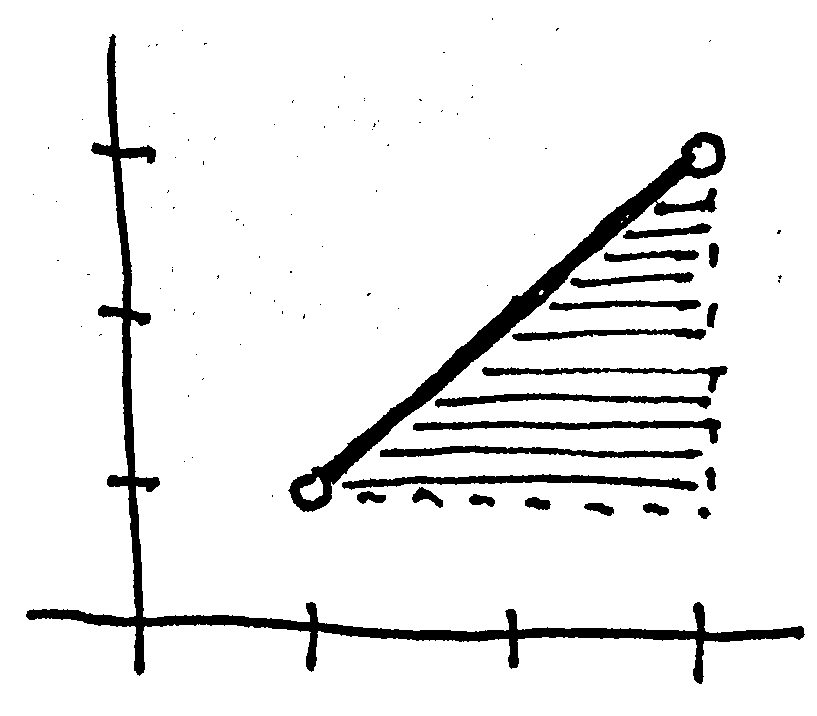
\includegraphics[height=2cm]{2021-1-C3/20210908_C_7.pdf}},
  %
  \quad
  %
  % (find-latexscan-links "C3" "20210908_C_9")
  % (find-xpdf-page "~/LATEX/2021-1-C3/20210908_C_9.pdf")
  C_9 \;=\;
  \vc{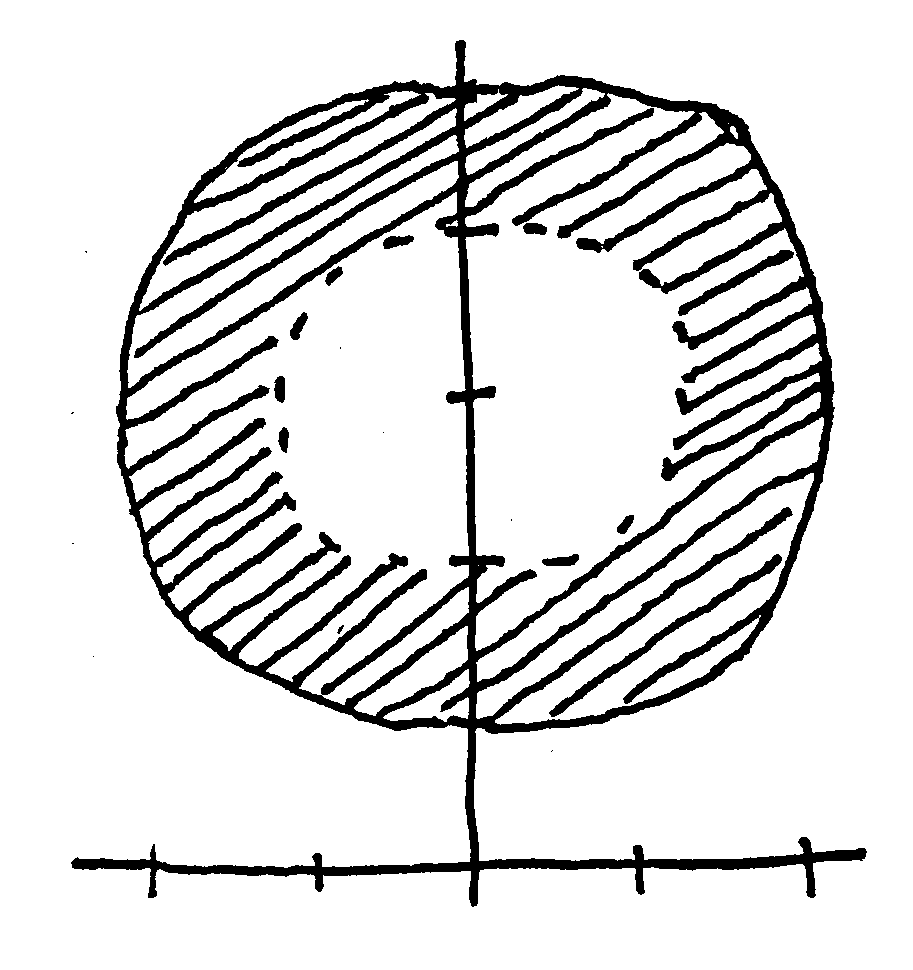
\includegraphics[height=2cm]{2021-1-C3/20210908_C_9.pdf}}.
$$

\newpage

% «exercicios-1-e-2»  (to ".exercicios-1-e-2")
% (c3m222topp 4 "exercicios-1-e-2")
% (c3m222topa   "exercicios-1-e-2")
% (c3m211afp 4 "exercicios-1-e-2")
% (c3m211afa   "exercicios-1-e-2")

{\bf Exercício 1.}

%\msk

Represente graficamente os conjuntos $C_1, \ldots, C_6$.

\bsk


{\bf Exercício 2.}

%\msk

Represente os conjuntos $C_7$, $C_8$, $C_9$

em ``notação de conjuntos'' --- isto é,

na forma $\setofxyst{\ldots}$.


\newpage

% «bolas»  (to ".bolas")
% (c3m211afp 5 "bolas")
% (c3m211afa   "bolas")

{\bf Bolas abertas e fechadas}

Se $P$ é um ponto de $\R^n$ então a

{\sl bola fechada de raio $ε$ em torno de $P$}, $\BF_ε(P)$, e a

{\sl bola aberta de raio $ε$ em torno de $P$}, $\BA_ε(P)$,

são definidas assim:
%
$$\begin{array}{rcl}
  \BF_ε(P) &=& \setofst{Q∈\R^n}{d(P,Q)≤ε} \\
  \BA_ε(P) &=& \setofst{Q∈\R^n}{d(P,Q)<ε} \\
  \end{array}
$$

\msk

Por exemplo, se $P=6∈\R^1$ então:
%
$$\scalebox{0.85}{$
  \begin{array}{rcl}
  \BF_2(6) &=& \setofst{Q∈\R^1}{d(6,Q)≤2} \\
           &=& \setofst{x∈\R}{d(6,x)≤2} \\
           &=& \setofst{x∈\R}{\sqrt{(6-x)^2}≤2} \\
           &=& \setofst{x∈\R}{      |x-6|   ≤2} \\
           &=& \setofst{x∈\R}{-2 ≤   x-6    ≤2} \\
           &=& \setofst{x∈\R}{-2+6 ≤ x      ≤2+6} \\
           &=& [4,8] \\
  \end{array}
  $}
$$

\newpage

% «exercicio-3»  (to ".exercicio-3")
% (c3m211afp 6 "exercicio-3")
% (c3m211afa   "exercicio-3")

{\bf Exercício 3.}

Represente graficamente:

\msk

a) $\BF_1((2,2))$,

b) $\BA_1((2,2))$.

\msk

Dica: estes conjuntos vão parecer muito mais com

``bolas de verdade'' do que o conjunto $\BF_2(6)$ do

slide anterior.

\bsk

Lembre que a gente desenha a fronteira de um conjunto

tracejada quando a gente quer indicar que os pontos da

fronteira não pertencem ao conjunto e a gente desenha

ela sólida quando quer indicar que os pontos dela

pertencem ao conjunto. Veja os desenhos dos

conjuntos $C_8$ e $C_9$.


\newpage

% «exercicio-4»  (to ".exercicio-4")
% (c3m211afp 7 "exercicio-4")
% (c3m211afa   "exercicio-4")

{\bf Exercício 4.}

Aqui você vai ter que ser capaz de visualizar bolas sobrepostas

a conjuntos que você já desenhou sem desenhar estas bolas.

Diga se cada uma das afirmações abaixo é verdadeira ou falsa.

\msk

a) $\BA_{0.1} ((0, 2.5))⊆C_1$

b) $\BA_{0.5} ((0, 2.5))⊆C_1$

c) $\BF_{0.5} ((0, 2.5))⊆C_1$

d) $\BA_{0.1} ((1, 3))⊆C_2$

e) $\BA_{0.1} ((2.5, 2.5))⊆C_2$

f) $\BA_{1} ((2, 2))⊆C_3$

g) $\BF_{1} ((2, 2))⊆C_3$

h) $\BA_{0.5} ((1, 0.5))⊆C_4$

i) $\BA_{0.1} ((0.5, 2))⊆C_5$

j) $\BA_{0.001} ((1.1, 1.01))⊆C_8$

\newpage

% «interior»  (to ".interior")
% (c3m222topp 9 "interior")
% (c3m222topa   "interior")
% (c3m211afp 8 "interior")
% (c3m211afa   "interior")

{\bf O interior de um conjunto (e conjuntos abertos)}

Def: o {\sl interior} de um conjunto $A⊂\R^n$, $\Int(A)$,

é definido como:
%
$$\Int(A) \;\;=\;\; \setofst{P∈A}{∃ε>0.\, \BA_ε(P)⊆A}.$$

Note que isto sempre é verdade: $\Int(A)⊂A$.

Dizemos que um conjunto $A$ é {\sl aberto} quando $A⊂\Int(A)$.



\newpage

% «infinitas-bob»  (to ".infinitas-bob")
% (c3m222topp 10 "infinitas-bob")
% (c3m222topa    "infinitas-bob")

{\bf Infinitas operações / seja com o Bob}

Pra entender a definição de interior e as próximas você vai precisar
fazer um número infinito de operações pra chegar no resultado, e pra
isso você vai ter que usar algumas técnicas que nós vimos em Cálculo 2
no semestre passado. Os links abaixo vão pras versões deste semestre
do material sobre essas técnicas, que ficou bem melhor do que o do
semestre passado.

\msk

Veja este PDF, a partir da página 11 dele:

{\footnotesize

% (c2m222srp 11 "set-comprehensions")
% (c2m222sra    "set-comprehensions")
%    http://angg.twu.net/LATEX/2022-2-C2-somas-de-riemann.pdf
\url{http://angg.twu.net/LATEX/2022-2-C2-somas-de-riemann.pdf}

}

\ssk

e relembre as definições de inf e sup daqui:

{\footnotesize

% (c2m222tfcsp 1)
%    http://angg.twu.net/LATEX/2022-2-C2-TFC1-e-TFC2.pdf
\url{http://angg.twu.net/LATEX/2022-2-C2-TFC1-e-TFC2.pdf}

}



% (c2m222tfcsp 1 "title")
% (c2m222tfcsa   "title")






\newpage

% «exercicio-5»  (to ".exercicio-5")
% (c3m211afp 9 "exercicio-5")
% (c3m211afa   "exercicio-5")

{\bf Exercício 5.}

Seja $A = [2,4] ⊂ \R^1$.

Verifique que $A$ não é aberto usando

a definição do slide anterior.

Dica: como $A = [2,4]$,
%
\def\iff{\Leftrightarrow}
%
$$\begin{array}{lrcl}
                 & A & \multicolumn{2}{l}{\text{não é aberto}} \\ 
   \iff \ph{m}   & A & \not⊂ & \Int(A) \\
   \iff          & A & \not⊂ & \setofst{P∈A}{∃ε>0.\, \BA_ε(P)⊆A} \\
   \iff          & [2,4] & \not⊂ & \setofst{P∈[2,4]}{∃ε>0.\, \BA_ε(P)⊆[2,4]} \\
  \end{array}
$$

\msk

Tente continuar você mesmo usando ou matematiquês ou português.

Você talvez vá precisar de truques que as pessoas costumam aprender

nos primeiros semestres mas acabaram não aprendendo dessa vez

por causa da pandemia...

\newpage

% «exercicio-6»  (to ".exercicio-6")
% (c3m211afp 10 "exercicio-6")
% (c3m211afa    "exercicio-6")

{\bf Exercício 6.}

\ssk

Represente graficamente:

\ssk

a) $\Int(C_8)$,

b) $\Int(C_4)$,

c) $\Int(C_5)$,

d) $\Int(\BA_1((2,2)))$.

\newpage

% «fecho»  (to ".fecho")
% (c3m211afp 11 "fecho")
% (c3m211afa    "fecho")

{\bf O fecho de um conjunto (e conjuntos fechados)}

Def: o {\sl fecho} de um conjunto $A⊂\R^2$, $\ovl{A}$,

é definido como:
%
$$\ovl{A} \;\;=\;\; \setofst{P∈\R^2}{∀ε>0.\, \BA_ε(P)∩A \neq ∅}$$

Compare com a definição do interior:
%
$$\Int(A) \;\;=\;\; \setofst{P∈A}{∃ε>0.\, \BA_ε(P)⊆A}.$$

Isto aqui sempre é verdade: $A ⊂ \ovl{A}$.

Quando $\ovl{A} ⊂ A$ dizemos que $A$ é um conjunto {\sl fechado}.


\newpage

% «exercicio-7»  (to ".exercicio-7")
% (c3m211afp 12 "exercicio-7")
% (c3m211afa    "exercicio-7")
% (find-LATEXgrep "grep --color=auto -niH --null -e bounds 2022*.tex")

%L Pict2e.bounds = PictBounds.new(v(0,0), v(3,2))
%L spec   = "(1,1)o--(2,1)c"
%L pws    = PwSpec.from(spec)
%L curve  = pws:topict()
%L p = PictList { curve:prethickness("2pt") }
%L p:pgat("pgatc"):preunitlength("15pt"):sa("Exercicio 7"):output()
\pu

{\bf Exercício 7.}

\unitlength=20pt

Digamos que:
%
$$D_1 \;\;=\;\;
  \ga{Exercicio 7}
$$

\msk

Represente graficamente:

a) $\ovl{C_8}$

b) $\ovl{D_1}$

c) $\Int(D_1)$


\newpage

{\bf Um aviso sobre a P2 (de 2021.2)}

Em quase todos os problemas deste PDF é muito

mais fácil mostrar que uma resposta está errada

do que mostrar que ela está certa... e o método

pra mostrar que uma resposta está errada vai

ser um dos assuntos principais da P2.

\msk

% (Vou explicar ele daqui a pouco!)


\newpage

% «algumas-traducoes»  (to ".algumas-traducoes")
% (c3m211afp 14 "algumas-traducoes")
% (c3m211afa    "algumas-traducoes")

{\bf Algumas traduções}

\def\iff{\Leftrigharrow}

$$\begin{array}{rcl}
  A⊂B   &=&   ∀a∈A. a∈B \\
  A=B   &=&   (A⊂B)∧(B⊂A) \\
  ¬(P∧Q) &=& ¬P∨¬Q \\
  ¬(P∨Q) &=& ¬P∧¬Q \\
  ¬(∀a∈A.P(a)) &=& ∃a∈A.¬P(a) \\
  ¬(∃a∈A.P(a)) &=& ∀a∈A.¬P(a) \\
  x∈\setofst{a∈A}{P(a)} &=& x∈A∧P(x) \\
  ¬(P→Q) &=& P∧¬Q \\ \relax
  [20,42) &=& \setofst{x∈\R}{20≤x<42} \\
  20≤x<42 &=& 20≤x ∧ x<42 \\
  \end{array}
$$

\bsk

Lembra que `$∧$' é ``e'', `$∨$' é ``ou'', `$¬$' é ``não'', `$→$' é
``implica''.


\newpage

% «algumas-traducoes-2»  (to ".algumas-traducoes-2")
% (c3m211afp 15 "algumas-traducoes-2")
% (c3m211afa    "algumas-traducoes-2")

{\bf Alguns exemplos de traduções}

$$\begin{array}{l}
  [a,b] ⊂ [20, 42) \\
  = \;\; ∀x∈[a,b]. x∈[20, 42) \\
  = \;\; ∀x∈[a,b]. 20≤x<42 \\
  = \;\; ∀x∈\R. x∈[a,b] → 20≤x<42 \\
  = \;\; ∀x∈\R. a≤x≤b → 20≤x<42   \\[10pt]
  %
  ¬([a,b] ⊂ [20, 42)) \\
  = \;\; ¬(∀x∈\R. a≤x≤b → 20≤x<42) \\
  = \;\; ∃x∈\R. ¬(a≤x≤b → 20≤x<42) \\
  = \;\; ∃x∈\R. ¬(a≤x≤b)∧(20≤x<42) \\
  = \;\; ∃x∈\R. ¬(a≤x ∧ x≤b)∧(20≤x<42) \\
  = \;\; ∃x∈\R. (¬(a≤x) ∨ ¬(x≤b))∧(20≤x<42) \\
  = \;\; ∃x∈\R. (x<a ∨ b<x)∧(20≤x<42) \\
  \end{array}
$$


% (c3q192 18 "20190920" "Subconjuntos de R2; fecho e interior")
% (c3q192 19 "20190926" "Abertos e fechados; imagem inversa; Teorema de Weierstrass; triangulo e xy")
% (c3q192 20 "20190927" "Mais imagem inversa e Teorema de Weierstrass")

% (find-bortolossi4page)
% (find-bortolossi4page (+ -120 121) "Cap 4")
% (find-bortolossi4page (+ -120 121) "4.1. Porque contínuas são importantes")
% (find-bortolossi4page (+ -120 123) "4.2. Continuidade em várias variáveis")
% (find-bortolossi4page (+ -120 129) "4.3. Weierstrass em n variáveis")
% (find-bortolossi4page (+ -120 139)   "distância euclidiana")
% (find-bortolossi4page (+ -120 142)   "bola aberta")
% (find-bortolossi4page (+ -120 142)   "bola fechada")
% (find-bortolossi4page (+ -120 143)   "conjunto limitado")
% (find-bortolossi4page (+ -120 143)   "ponto de fronteira")
% (find-bortolossi4page (+ -120 144)   "fronteira de um conjunto")
% (find-bortolossi4page (+ -120 145)   "conjunto fechado")
% (find-bortolossi4page (+ -120 146)   "conjunto compacto")
% (find-bortolossi4page (+ -120 147)   "o teorema de Weierstrass")
% (find-bortolossi4page (+ -120 148)   "ponto interior")
% (find-bortolossi4page (+ -120 148)   "conjunto aberto")
% (find-bortolossi4page (+ -120 151) "4.4. Exercícios")


\newpage

% «algumas-nots-novas»  (to ".algumas-nots-novas")
% (c3m222topp 10 "algumas-nots-novas")
% (c3m222topa    "algumas-nots-novas")

{\bf Imagem inversa}

\scalebox{0.55}{\def\colwidth{9cm}\firstcol{

Algumas das igualdades abaixo são definições,

as outras são exemplos.
%
$$\begin{array}{rcl}
  H(x,y)    &=& xy \\
  H_I       &=& \setofxyst{H(x,y)∈I} \\
  H_{[a,b]} &=& \setofxyst{H(x,y)∈[a,b]} \\
  H_{[0,1]} &=& \setofxyst{H(x,y)∈[0,1]} \\
  H^{-1}(a) &=& \setofxyst{H(x,y)=a} \\
  H^{-1}(I) &=& \setofxyst{H(x,y)∈I} \\
  H^{-1}([0,1]) &=& \setofxyst{H(x,y)∈[0,1]} \\
                &=& H_{[0,1]} \\
  \end{array}
$$

\bsk

{\bf Exercício 8.}

Represente graficamente:
%
$$\begin{array}{rcl}
  C_{1} &=& H^{-1}(0) \\
  C_{2} &=& H^{-1}(1) \\
  C_{3} &=& H^{-1}([0,1]) \\
  C_{4} &=& H^{-1}((0,1))\\
  C_{5} &=& \Int(C_3)\\
  C_{6} &=& \overline{C_4} \\
  C_{7} &=& H^{-1}(4) \\
  C_{8} &=& H^{-1}([0,4]) \\
  C_{9} &=& \setofxyst{1≤x \text{ e } 1≤y} \\
  C_{10} &=& C_8∩C_9 \\
  \end{array}
$$


}\anothercol{

{\bf Conjuntos limitados e compactos}

Um conjunto $C∈\R^2$ é {\sl limitado} quando ele

obedece isto:
%
$$∃r∈\R.\,C⊂B_r((0,0))$$.

Um conjunto $C∈\R^2$ é {\sl compacto} quando ele é

fechado e limitado.




\bsk
\bsk
\bsk

{\bf Exercício 9.}

Preencha a tabela abaixo com `$\True$'s e `$\False$'s.

\bsk

$\begin{array}{lcccccccccc}
   & C_1
   & C_2
   & C_3
   & C_4
   & C_5
   & C_6
   & C_7
   & C_8
   & C_{10} \\
   \text{é aberto} \\
   \text{é fechado} \\
   \text{é limitado} \\
   \text{é compacto} \\
 \end{array}
$

}}


\newpage

% «maximos-numa-elipse»  (to ".maximos-numa-elipse")
% (c3m222topp 19 "maximos-numa-elipse")
% (c3m222topa    "maximos-numa-elipse")
{\bf Máximos numa elipse}


\scalebox{0.52}{\def\colwidth{11cm}\firstcol{

Dê uma olhada nas figuras das páginas 355 e 356 do Bortolossi,

no capítulo 10 dele:

\ssk

{\scriptsize

% (find-books "__analysis/__analysis.el" "bortolossi")
% (find-books "__analysis/__analysis.el" "bortolossi" "na borda da elipse")
% (find-bortolossi10page (+ -350 355)   "máximos de x^2+y^2 numa elipse")
% (find-bortolossi10page (+ -350 356)   "máximos de x^2+y^2 na borda da elipse")
%    http://angg.twu.net/2019.2-C3/Bortolossi/bortolossi-cap-10.pdf
\url{http://angg.twu.net/2019.2-C3/Bortolossi/bortolossi-cap-10.pdf\#page=5}

\url{http://angg.twu.net/2019.2-C3/Bortolossi/bortolossi-cap-10.pdf\#page=6}

}

Ele usa:
%
$$\begin{array}{rcl}
  f(x,y) &=& x^2+y^2 \\
  g(x,y) &=& \frac{x^2}{4}+\frac{y^2}{9} \\
  D_2 &=& \setofxyst{g(x,y)≤1} \\
  D_3 &=& \setofxyst{g(x,y)=1} \\
  \end{array}
$$

$D_2$ é uma elipse ``cheia'' incluindo o interior dela, e

$D_3$ é só a fronteira de $D_2$.

Note que $(-2,0),(2,0),(0,3),(0,-3)∈D_3$.

\bsk

{\bf Exercício 10.}

a) Desenhe algumas curvas de nível de $f(x,y)$.

\msk

b) Na página 354 o Bortolossi desenha curvas de nível
dentro de um quadrado. Desenhe algumas curvas de nível
de $f(x,y)$ dentro da ``elipse cheia'' $D_2$.

\msk

c) Tente descobrir {\sl no olhômetro} quais são os máximos
e mínimos de $f(x,y)$ em $D_2$. Dica: o Bortolossi leva
várias páginas fazendo isso --- leia o texto dele!


}\anothercol{

  {\bf Dica:} o objetivo do item (c) é você aprender a resolver só com
  curvas de nível as idéias que o Bortolossi apresenta usando figuras
  em 3D. Se você não conseguir fazer a tradução das figuras 3D pra
  curvas de nível direto você pode começar desenhando ``cortes'' sobre
  as figuras 3D, como na questão do mini-teste 1 de 2020.2:

\ssk

{\scriptsize

% (c3m202tudop 83 "title")
% (c3m202tudoa   "title")
%    http://angg.twu.net/LATEX/2020-2-C3-tudo.pdf#page=83
\url{http://angg.twu.net/LATEX/2020-2-C3-tudo.pdf\#page=83}

}

\bsk


...e repare que quando o Bortolossi chega no capítulo 12 ele passa a
usar quase só curvas de nível e gradientes --- ele praticamente
abandona as figuras 3D:

\ssk

{\scriptsize

% (find-books "__analysis/__analysis.el" "bortolossi")
% (find-books "__analysis/__analysis.el" "bortolossi" "12. Otimização com")
%    http://angg.twu.net/2019.2-C3/Bortolossi/bortolossi-cap-12.pdf
\url{http://angg.twu.net/2019.2-C3/Bortolossi/bortolossi-cap-12.pdf}

}



}}





\GenericWarning{Success:}{Success!!!}  % Used by `M-x cv'

\end{document}

%  ____  _             _         
% |  _ \(_)_   ___   _(_)_______ 
% | | | | \ \ / / | | | |_  / _ \
% | |_| | |\ V /| |_| | |/ /  __/
% |____// | \_/  \__,_|_/___\___|
%     |__/                       
%
% «djvuize»  (to ".djvuize")
% (find-LATEXgrep "grep --color -nH --null -e djvuize 2020-1*.tex")

 (eepitch-shell)
 (eepitch-kill)
 (eepitch-shell)
# (find-fline "~/2022.2-C3/")
# (find-fline "~/LATEX/2022-2-C3/")
# (find-fline "~/bin/djvuize")

cd /tmp/
for i in *.jpg; do echo f $(basename $i .jpg); done

f () { rm -v $1.pdf;  textcleaner -f 50 -o  5 $1.jpg $1.png; djvuize $1.pdf; xpdf $1.pdf }
f () { rm -v $1.pdf;  textcleaner -f 50 -o 10 $1.jpg $1.png; djvuize $1.pdf; xpdf $1.pdf }
f () { rm -v $1.pdf;  textcleaner -f 50 -o 20 $1.jpg $1.png; djvuize $1.pdf; xpdf $1.pdf }

f () { rm -fv $1.png $1.pdf; djvuize $1.pdf }
f () { rm -fv $1.png $1.pdf; djvuize WHITEBOARDOPTS="-m 1.0 -f 15" $1.pdf; xpdf $1.pdf }
f () { rm -fv $1.png $1.pdf; djvuize WHITEBOARDOPTS="-m 1.0 -f 30" $1.pdf; xpdf $1.pdf }
f () { rm -fv $1.png $1.pdf; djvuize WHITEBOARDOPTS="-m 1.0 -f 45" $1.pdf; xpdf $1.pdf }
f () { rm -fv $1.png $1.pdf; djvuize WHITEBOARDOPTS="-m 0.5" $1.pdf; xpdf $1.pdf }
f () { rm -fv $1.png $1.pdf; djvuize WHITEBOARDOPTS="-m 0.25" $1.pdf; xpdf $1.pdf }
f () { cp -fv $1.png $1.pdf       ~/2022.2-C3/
       cp -fv        $1.pdf ~/LATEX/2022-2-C3/
       cat <<%%%
% (find-latexscan-links "C3" "$1")
%%%
}

f 20201213_area_em_funcao_de_theta
f 20201213_area_em_funcao_de_x
f 20201213_area_fatias_pizza



%  __  __       _        
% |  \/  | __ _| | _____ 
% | |\/| |/ _` | |/ / _ \
% | |  | | (_| |   <  __/
% |_|  |_|\__,_|_|\_\___|
%                        
% <make>

 (eepitch-shell)
 (eepitch-kill)
 (eepitch-shell)
# (find-LATEXfile "2019planar-has-1.mk")
make -f 2019.mk STEM=2022-2-C3-topologia veryclean
make -f 2019.mk STEM=2022-2-C3-topologia pdf

% Local Variables:
% coding: utf-8-unix
% ee-tla: "c3to"
% ee-tla: "c3m222top"
% End:
